\chapter{Model Selection}\label{model_selection}

Since our study involves working with a formula for the interaction-based sentiment analysis, and a pre-trained model for the Natural Language Processing task, we do not use any specific machine learning model. Even though our work involves working with Banglish text, we chose the Bangla text-based model of BanglaBERT due to its higher BLUB Score. From the table \ref{banglabert_performance} collected from BanglaBERT paper \cite{banglabert}, we can see that the performance of the BanglaBERT model exceeds that of the BanglishBERT one.

\begin{figure}[H]
    \begin{center}
        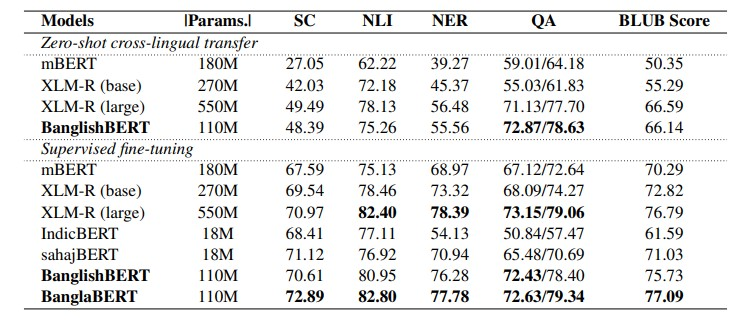
\includegraphics[width=0.8 \linewidth]{figures/banglabert_models.jpg}
    \end{center}
    \caption{Performance Comparison of Different Pretrained NLP Models for Different Downstream Tasks}
    \label{banglabert_performance}
\end{figure}

BanglaBERT offers three pre-trained models for the downstream task of the Bangla language. Due to the limitation of computation hardware and resources, we chose to work with the 'BanglaBERT Base' model. The pre-trained weights of the model were downloaded from HuggingFace model hub \footnote{https://huggingface.co/csebuetnlp}. For fine-tuning the model, we used the \texttt{sequence\_classification.py} script provided with the model's codebase.